% TRACE-rPPG extended abstract, NSysS 2026 poster track.
% Generated by scripts/build_deliverables.py from results files; edit the
% template (template_abstract.tex), not this output. Compile on Overleaf
% with the IEEEtran class; figures are in ./figures.
\documentclass[conference]{IEEEtran}
\usepackage{graphicx}
\usepackage{booktabs}
\usepackage{amsmath}
\usepackage{url}

\begin{document}

\title{Does Video Compression Widen the Skin-Tone Gap in Remote Photoplethysmography? A Simulated Pilot and a Classical Mitigation}

\author{\IEEEauthorblockN{Ahammad Shawki \and S. M. Abu Fayeem}
\IEEEauthorblockA{[Department, University], Dhaka, Bangladesh\\
[emails]}}

\maketitle

\begin{abstract}
Remote photoplethysmography (rPPG) estimates heart rate from the colour change each heartbeat causes in facial skin. It is known to be less accurate on darker skin, and separately known to degrade under video compression, but the interaction has not been measured. Because bitrate is a network-layer decision, an interaction would mean that constrained connections compound a demographic disadvantage. We build a fully classical pipeline (convolution filtering, Fourier spectra, no learned estimator), a compression harness with lossless controls, and a face-video simulator with controllable melanin, and run a pilot of 36 simulated volunteers across H.264, H.265, VP9 at 100, 200, 400, 800, 1600 kbps. Compression did not widen the skin-tone gap. Darker skin was already near its failure plateau at every bitrate, and compression dragged lighter skin down to meet it. We also evaluate TRACE, a signal-quality-adaptive fusion of classical methods with a pulse-blind artifact reference, and two pretrained neural baselines. All results are simulated; the protocol for recorded participants is ready.
\end{abstract}

\section{Motivation and Gap}
Chrominance rPPG methods degrade on Fitzpatrick V to VI skin \cite{dasari2021,nowara2020}, and compression measurably damages rPPG \cite{mcduff2017,nowara2019}. The field names both factors as separately studied. An OpenAlex search (2,023 rPPG papers; 51 on compression, 121 on skin tone) found 3 papers mentioning both and none measuring the interaction. Melanin absorbs more light, so the pulse is a smaller change in pixel levels on darker skin; codecs subsample chroma and quantise small temporal changes. A weaker signal should cross the codec noise floor at a higher bitrate, making the disparity multiplicative rather than additive.

\section{Method}
\textbf{Pipeline.} Haar face detection with phase-correlation tracking (the Fourier shift theorem; re-detecting every few frames made the box wobble enough to destroy the pulse on dark skin); forehead and cheek means with an adaptive chroma mask; moving-average detrending and a hand-built windowed-sinc bandpass (0.7 to 4 Hz), both convolutions; green, CHROM \cite{dehaan2013} and POS \cite{wang2017}; a windowed FFT with parabolic peak interpolation and a sub-harmonic check.

\textbf{TRACE.} Each method is scored by the fraction of in-band spectral power at its peak and harmonic. Scores alone failed on held-out data (periodic motion is also a concentrated peak), so a pulse-blind artifact reference was added: normalised RGB along the brightness direction with a nominal pulse direction removed. Its spectrum masks each method's spectrum ($(1-A(f))^{k}$, $k=4.0$) and penalises a method whose peak coincides with artifact power; spectra are fused with weights $q^{\gamma}$, $\gamma=1.0$, and a reading below quality 0.24 is reported as low confidence. Parameters were tuned on 48 simulated subjects and frozen before testing.

\textbf{Simulator and harness.} A public-domain portrait is rendered at 640x480, 30 fps with a two-layer reflectance model: melanin attenuates light with wavelength-dependent absorption, surface reflection is channel neutral, plus motion, lighting drift, chromatic screen light and sensor noise, and a heartbeat with known beat times. Codecs, detector and pipeline are real. Every condition re-encodes the same lossless source; controls separate colour conversion (YUV 4:4:4), chroma subsampling (4:2:0) and quantisation. The lossless control decodes bit-identically.

\textbf{Statistics.} Per-subject, per-condition MAE is modelled as $\text{err} \sim \log_2(\text{kbps}) \times \text{dark} + (1 \mid \text{subject})$; the interaction coefficient, with Wald and subject-bootstrap intervals, is the claim.

\section{Results (simulated)}
\begin{figure}[t]
\centering
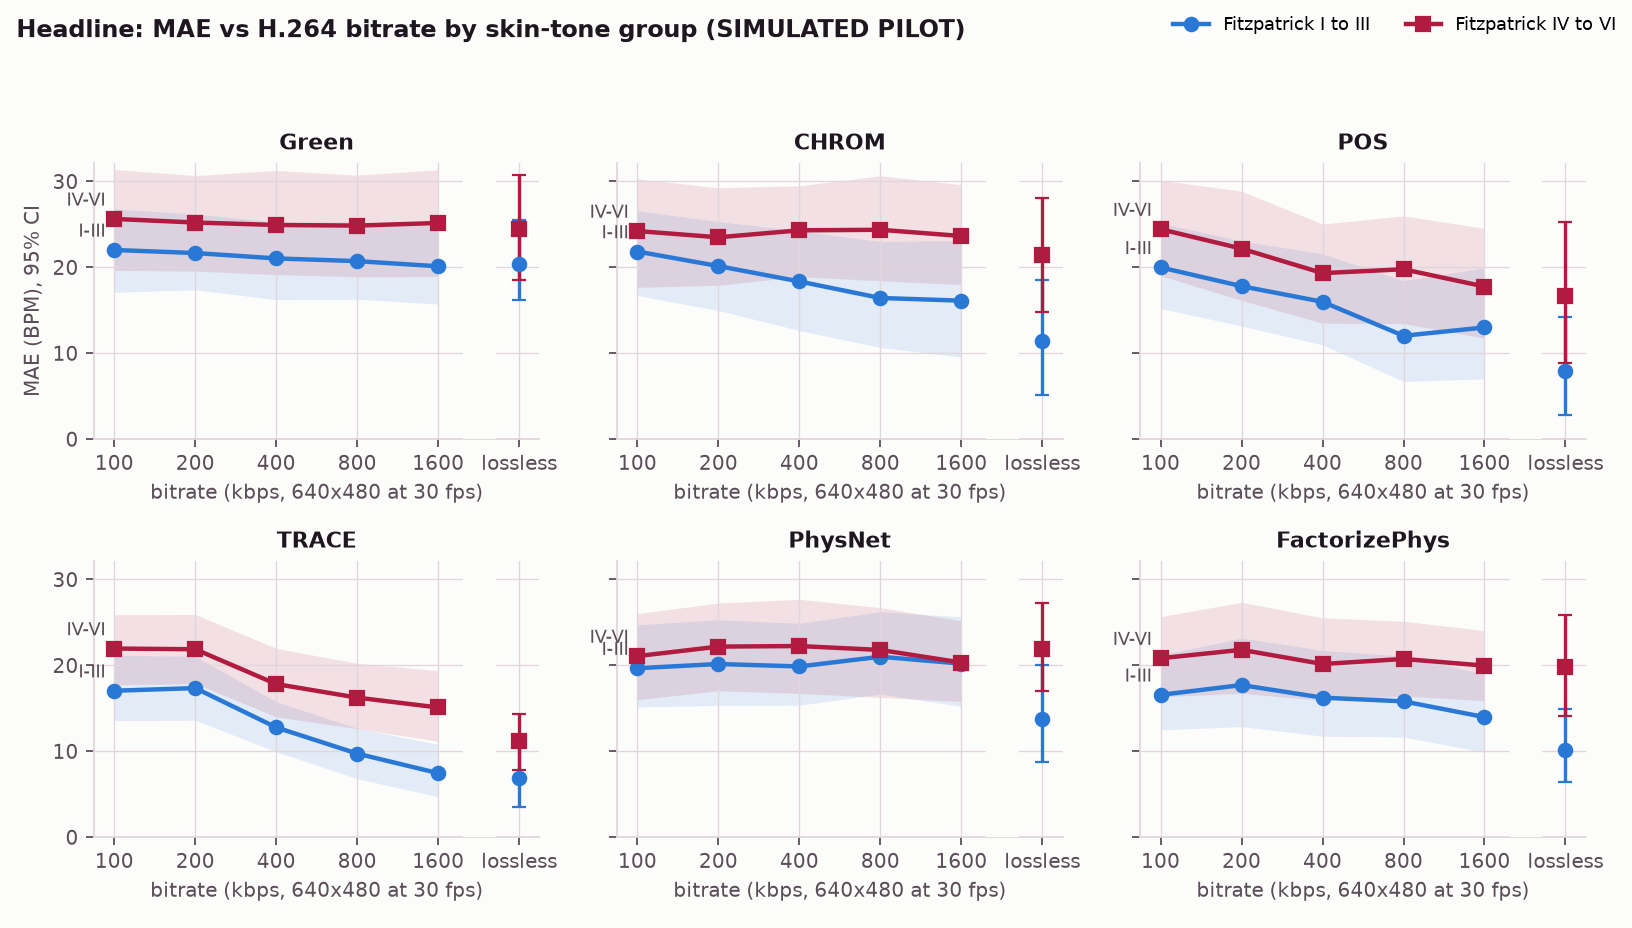
\includegraphics[width=\linewidth]{figures/fan_h264.png}
\caption{MAE against H.264 bitrate for lighter (I to III) and darker (IV to VI) simulated skin. Lossless at right.}
\label{fig:fan}
\end{figure}

Fig.~\ref{fig:fan} shows the headline grid. For POS under H.264, the dark-minus-light error gap was 8.8 BPM on lossless video and 4.4 BPM at 100 kbps. The interaction coefficient was 0.40 BPM per doubling of bitrate (95\% CI -0.57 to 1.37, p = 0.420; subject bootstrap -0.77 to 1.65). The interval includes zero: in this sample the curves do not fan apart detectably. Windows within 5 BPM: 79\% lighter vs 56\% darker on lossless video, 18\% vs 15\% at 100 kbps. For CHROM: For CHROM under H.264, the dark-minus-light error gap was 10.0 BPM on lossless video and 2.4 BPM at 100 kbps. The interaction coefficient was 1.49 BPM per doubling of bitrate (95\% CI 0.77 to 2.21, p < 0.001; subject bootstrap 0.43 to 2.35). The gap narrowed as bitrate fell, the opposite of the hypothesis. Windows within 5 BPM: 66\% lighter vs 25\% darker on lossless video, 14\% vs 9\% at 100 kbps. Darker skin was already near its failure plateau at every bitrate, and compression pulled lighter skin down to meet it: the narrowing reflects convergence at failure, not a benefit to darker skin. On a still face, the correlation of the decoded skin trace with the true pulse fell from 0.92 (lighter) and 0.84 (darker) on lossless video to 0.46 and -0.11 at 100 kbps H.264.

\textbf{Mitigation.} On the full grid the lowest error on lossless video came from TRACE (9.0 BPM) and at 400 kbps from TRACE (15.3). TRACE scored 9.0 and 15.3; POS 12.2 and 17.7; POS with the artifact mask alone 9.1 and 16.1; FactorizePhys 15.0 and 18.2. TRACE's lossless skin-tone gap was 4.3 BPM against 8.8 for POS. On a separate held-out uncompressed cohort, POS scored 11.8 BPM, POS with the artifact mask alone 7.3, and TRACE 9.7; readings TRACE marked confident (93\% of windows) had 8.7 BPM error against 22.8 for flagged ones.

\textbf{Learned baselines.} PhysNet and FactorizePhys (rPPG-Toolbox \cite{liu2023}, trained on PURE): For FactorizePhys under H.264, the dark-minus-light error gap was 9.6 BPM on lossless video and 4.3 BPM at 100 kbps. The interaction coefficient was 0.43 BPM per doubling of bitrate (95\% CI -0.15 to 1.01, p = 0.145; subject bootstrap -0.06 to 0.94). The interval includes zero: in this sample the curves do not fan apart detectably. Windows within 5 BPM: 60\% lighter vs 27\% darker on lossless video, 24\% vs 15\% at 100 kbps.

\section{Limitations and Next Steps}
Skin-tone physics is modelled, so the simulated result is evidence about the mechanism, not about people. The next step is recording Fitzpatrick III to VI volunteers in Dhaka losslessly with a pulse oximeter; the pilot's variance components give more than 40 participants per group for 80\% power at 1.0 BPM per doubling. Heart-rate variability outputs are wellness indicators, not diagnoses.

\begin{thebibliography}{9}
\bibitem{dasari2021} A. Dasari, S. K. A. Prakash, L. A. Jeni, C. S. Tucker, ``Evaluation of biases in remote photoplethysmography methods,'' \emph{npj Digit. Med.}, 4:91, 2021.
\bibitem{nowara2020} E. M. Nowara, D. McDuff, A. Veeraraghavan, ``A meta-analysis of the impact of skin tone and gender on non-contact photoplethysmography measurements,'' CVPR Workshops, 2020.
\bibitem{mcduff2017} D. McDuff, E. B. Blackford, J. R. Estepp, ``The impact of video compression on remote cardiac pulse measurement using imaging photoplethysmography,'' IEEE FG, 2017.
\bibitem{nowara2019} E. M. Nowara, D. McDuff, ``Combating the impact of video compression on non-contact vital sign measurement using supervised learning,'' ICCV Workshops, 2019.
\bibitem{dehaan2013} G. de Haan, V. Jeanne, ``Robust pulse rate from chrominance-based rPPG,'' \emph{IEEE Trans. Biomed. Eng.}, 60(10), 2013.
\bibitem{wang2017} W. Wang, A. C. den Brinker, S. Stuijk, G. de Haan, ``Algorithmic principles of remote PPG,'' \emph{IEEE Trans. Biomed. Eng.}, 64(7), 2017.
\bibitem{liu2023} X. Liu et al., ``rPPG-Toolbox: Deep remote PPG toolbox,'' NeurIPS Datasets and Benchmarks, 2023.
\end{thebibliography}

\end{document}
